%% Author_tex.tex
%% V1.0
%% 2012/13/12
%% developed by Techset
%%
%% This file describes the coding for rsproca.cls

\documentclass[]{rsos}%%%%where rsos is the template name

%%%% *** Do not adjust lengths that control margins, column widths, etc. ***

\usepackage{color}
\usepackage[table,dvipsnames]{xcolor}
\definecolor{mygray}{gray}{0.6}


%%%%%%%%%%% Defining Enunciations  %%%%%%%%%%%
\newcommand{\arxiv}{arXiv}
%%%%%%%%%%%%%%%%%%%%%%%%%%%%%%%%%%%%%%%%%%%%%%%
\usepackage[normalem]{ulem}
\newcommand{\del}[1]{\textcolor{red}{\sout{#1}}}
\newcommand{\add}[1]{\textcolor{blue}{#1}}
\newcommand{\todo}[1]{\textcolor{green}{#1}}

%\newcommand{\del}[1]{}
%\newcommand{\add}[1]{#1}

\begin{document}

%%%% Article title to be placed here
\title{The impact of the COVID-19 pandemic on academic productivity}

\author{%%%% Author details
A. R. Casey$^{1,2}$,  I. Mandel$^{1,3,4}$ and P. K. Ray$^{5}$}

%%%%%%%%% Insert author address here
\address{$^1$School of Physics \& Astronomy, Monash University, Clayton 3800, Victoria, Australia\\
$^2$ARC Centre of Excellence for Astrophysics in Three Dimensions (ASTRO-3D), Australia\\
$^3$OzGrav, Australian Research Council Centre of Excellence for Gravitational Wave Discovery, Australia\\
$^4$Institute of Gravitational Wave Astronomy and School of Physics and Astronomy, University of Birmingham, Birmingham, B15 2TT, United Kingdom\\
$^5$Department of Mathematics, Imperial College London, London, United Kingdom
}

%%%% Subject entries to be placed here %%%%
\subject{xxxxx, xxxxx, xxxx}

%%%% Keyword entries to be placed here %%%%
\keywords{COVID, pre-print, academic productivity}

%%%% Insert corresponding author and its email address}
\corres{Andrew R. Casey\\
\email{andrew.casey@monash.edu}}

%%%% Abstract text to be placed here %%%%%%%%%%%%
\begin{abstract}
`Publish or perish’ is an expression describing the pressure on academics to consistently publish research to ensure a successful career in academia. 
With a global pandemic that has changed the world, how has it changed academic productivity? 
Here we show that academics are posting more papers on the arXiv pre-print server than would be expected had the pandemic not occurred: 341,474 pre-prints were posted between 2020-2021, up 14\% from 2019 and above the predictions of our Gaussian process model.
%168,630 were posted in 2020 , a +12.6\% change from 2019 and $+1.4\sigma$ deviation above the 162,577 predicted by our Gaussian process model. % todo: reword
We find that that most individual fields were not measurably affected by the pandemic.
However, we do observe a significant ongoing decline in general physics pre-prints, as well as temporary declines in areas of high-energy physics, where the cancellation of a key conference played a key role.
The most significant increase occurred in quantitative biology where a 50\%~increase ($+8\sigma$) in pre-prints posted in 2020 was driven by research related to the COVID-19 pandemic. 
Some of these `COVID papers' are by biologists using arXiv for the first time, but many are written by researchers from other fields (e.g., physicists, mathematicians). 
\end{abstract}
%%%%%%%%%%%%%%%%%%%%%%%%%%%

\maketitle

%%%%%%%%%% Insert the texts which can accomdate on firstpage in the tag "fmtext" %%%%%


\noindent Peer-reviewed publications are the most common measure of productivity in academia. The \arxiv\cite{Ginsparg:2011} ({https://arxiv.org}) is a service for the distribution of research publications (pre-prints) prior to their appearance in a journal. The presence of a pre-print on \arxiv\ does not ensure that the contents have passed peer-review, but most material on \arxiv\ eventually goes through peer-review because it is now standard in many research fields to post to \arxiv\ either during or after the peer-review process \cite{Lariviere:2014}. For this reason, the number of pre-prints posted to \arxiv\ approximates the number of peer-reviewed publications written in these fields.


Here we make quantitative comparisons on the number of pre-prints posted to \arxiv\ before and during the pandemic. It is important to recognise that the pandemic has affected both the general population\cite{Nicola:2020,Chu:2020,IbnMohammed:2021} and scientific community\cite{Viglione:2020,Gewen:2020,King:2021} in complex and unequal ways. Scientists have faced substantial challenges driven by a large number of factors including: generational inequality, carer responsibilities, modified work environments, and other personal and professional circumstances. Our analysis does not directly consider these important factors, nor does it account for groups or individuals disproportionately affected by the pandemic. We have instead adopted a broad perspective and present new quantitative results for entire scientific fields. The aim is to provide a “large-scale” view of scientific productivity which will serve as a foundation for future studies on the detailed impacts of COVID-19 on academic work.

We retrieved metadata for 1,660,423 pre-prints posted to \arxiv\ between 1 April 2007 and 31 May 2022. The metadata includes the creation date, research field(s), title, author name(s), abstract, and other miscellaneous information\cite{Clement:2019}. There is an increasing number of pre-prints posted to \arxiv\ each year in nearly every field (Figure~\ref{fig:1}). These long-term trends are relatively predictable from year to year, allowing us to quantify any change in academic productivity due to the COVID-19 pandemic. The number of pre-prints posted varies substantially by category. Computer science (\texttt{cs}) is the growing the fastest with more than 5,000 pre-prints per month, followed by math (\texttt{math}) with about 3,500 per month. For contrast, only $\approx$200 pre-prints are posted each month quantitative biology (\texttt{q-bio}), and just $\approx$40 in nuclear experimental physics (\texttt{nucl-ex}). For this reason, we model the number of monthly pre-prints in each research field separately. We used the number of publications from January 2015 to December 2019 to train a predictive Gaussian process model\cite{Rasmussen:2006}. This model treats the number of monthly pre-prints in a research field as a sequence of normally distributed random variables. The expected number of pre-prints was assumed to increase linearly with time, and a quasi-periodic kernel function\cite{Rasmussen:2006,Ambikasaran:2014} was used to capture seasonal variations (Figure~\ref{fig:1}). In nearly all research fields, the number of pre-prints posted since January 2020 agree closely with the model predictions (Table~1) indicating no significant overall decline in academic productivity due to the COVID-19 pandemic. %In fact, the total number of \arxiv\ pre-prints in 2020 across all fields (168,630) exceeds our model predictions ($162{,}577 \pm 4{,}393$; $+1.4\sigma$).  % todo

The exception is general physics (\arxiv\ category \texttt{physics}; not all physics-related domains), which shows the largest decline in pre-prints by number since the pandemic began. In 2020 the number posted to general physics actually exceeded our model predictions (15,242 compared to 14,746) by $1\sigma$, driven by a short peak of pre-prints posted to Physics and Society (\texttt{physics.soc-ph}) in early 2020. When we segment the number of pre-prints posted to physics by their sub-category we find that Computational Physics (\texttt{physics.comp-ph}) and Applied Physics (\texttt{physics.app-ph}) had significant drops in pre-print counts since the pandemic began (Figure~\ref{fig:physics}). All other physics sub-categories remained largely stable with time. The category of mathetmatical physics (\texttt{math-ph}) also showed a decline in pre-prints since the pandemic began, but this category has about an order of magnitude fewer pre-prints posted than physics. The mathematical physics category does not have defined sub-categories, making it more difficult to evaluate whether this decline occurred in particular areas of study.


Experimental research projects often require specialised laboratories, or data to be collected over many years. The pandemic has forced many laboratories to close or operate with restricted access\cite{PhysicsWorld,ScienceMag,Castelvecchi}, which could lead to long-lasting delays in ongoing experiments or immediate drops in publication rates in part due to difficulty in accessing completed (or nearly completed) experiment data. This could explain why there are declines in pre-prints in some sub-categories (e.g., Applied Physics), but there is not significant evidence of this in pre-print numbers of experimental-only fields (e.g., \texttt{hep-ex} or \texttt{nucl-ex}). In those fields the model predictions agree reasonably well with the pre-prints since 2020.




\begin{figure}[!h]
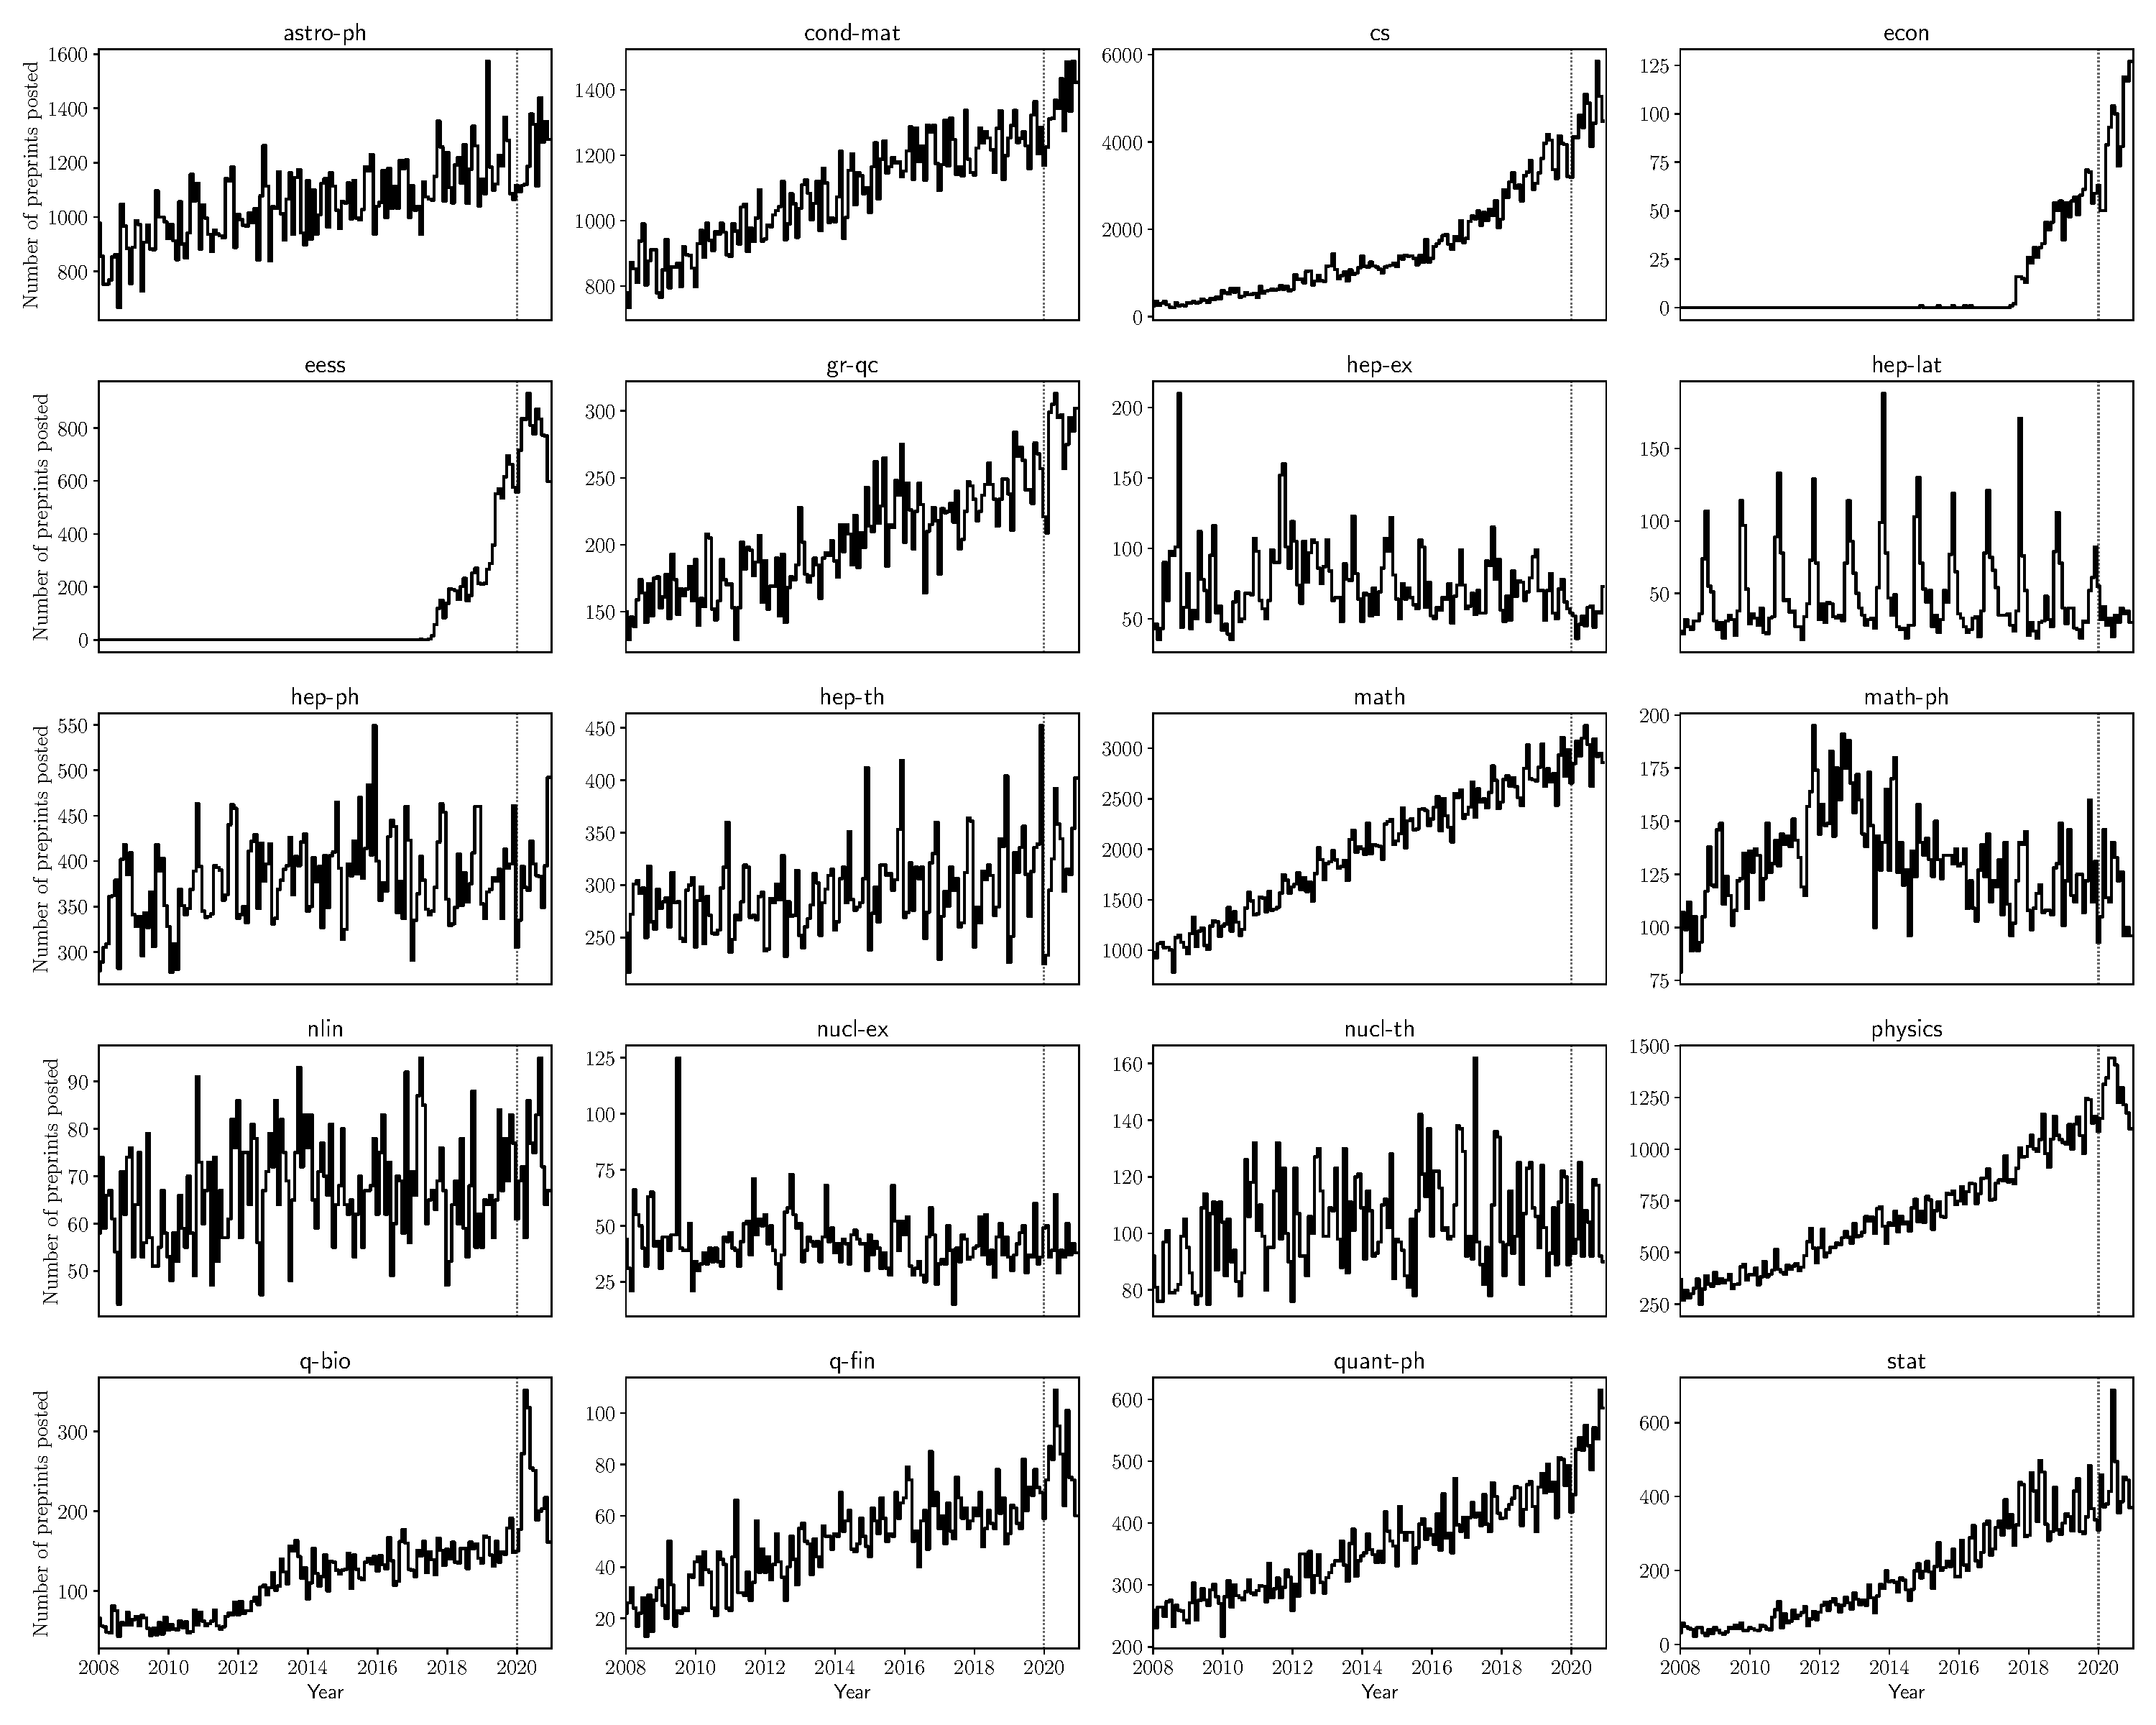
\includegraphics[width=0.95\linewidth]{pre-prints-segmented-by-field}
\caption{There has been no significant change in monthly \arxiv\ pre-prints (black) since the COVID-19 pandemic began. The expected number of pre-prints from our Gaussian Process model is shown in red, and the red region shows the uncertainty in that expectation. The blue line shows predictions from an autoregressive integrated moving average model.}
\label{fig:1}
\end{figure}



Border closures and travel restrictions forced many academic conferences to be held online-only, or to be cancelled. Hosting conferences online creates a mix of effects, as forgoing in-person experiences benefits those who could not otherwise participate due to visa issues or travel costs\cite{Guinnessy:2021}. The immediate impact of cancelling a conference is readily apparent in pre-print counts in lattice physics (Figure~\ref{fig:1}; \arxiv\ subject code \texttt{hep-lat}, see Methods), where most pre-prints are posted around December each year as conference proceedings from the International Symposium on Lattice Field Theory. In 2020 the conference was cancelled\cite{LatticeConferenceWebsite}, and no accompanying pre-prints exist. The conference was held in 2021 with nearly twice the number of corresponding authors than the 2019 conference\cite{LatticeConferenceWebsite2019,LatticeConferenceWebsite2021} (634 compared to 303), but the impact of conference cancellations and travel restrictions on academic research is likely to extend well beyond the output of a single field in a particular year, since discussions at conferences spark new research ideas and collaborations that can lead to publications many months or years later\cite{Wang:2017}.


%Throughout 2020, research in condensed matter (\texttt{cond-mat}) saw a $1.8\sigma$ increase above our model predictions (observed 16,188; predicted 15,325 $\pm$ 492). % todo: update for context of 2021
%Segmenting condensed matter pre-prints by research topic shows that most of this increase (in \texttt{cond-mat}) was driven by a 30\% increase in material science pre-prints (\texttt{cond-mat.mtrl-sci}). % todo:


%del{There is some evidence of this in pre-print numbers, with {20\%} fewer pre-prints in high energy physics (\texttt{hep-ex}) in 2020 than expected by our model (observed 615; predicted 818 $\pm$ 94)}
%\add{The number of pre-prints posted to \arxiv\ in the \texttt{physics} category spiked early in 2020, but the total number of physics pre-prints posted that year was only $1\sigma$ higher than the prediction from our model, because this spike was counter-balanced by a decline in the second half of 2020. This decline has steadily continued throughout 2021 and 2022, with physics showing the most significant decline in pre-prints since the pandemic began.}

%But declines are not ubiquitous across all experimental fields. The closest comparable field of phenomenology in high energy physics (\texttt{hep-ph}) showed no substantial decline. Neither did nuclear experimental research (\texttt{nucl-ex}). 


\begin{figure}[!t]
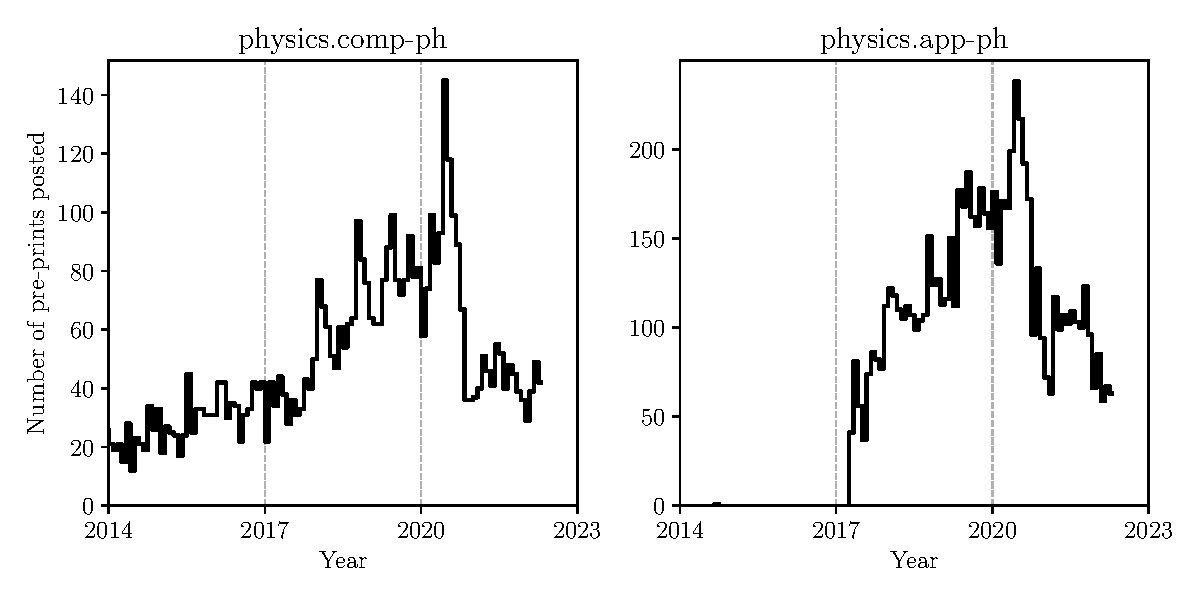
\includegraphics[width=0.95\linewidth]{physics-pre-prints}
\caption{The number of pre-prints posted to \arxiv\ in the categories of Computational Physics (\texttt{physics.comp-ph}) and Applied Physics (\texttt{physics.app-ph}). The decline in physics pre-prints since the pandemic began (Figure~\ref{fig:1}) is largely explained by the drop in pre-prints in Computational Physics and Applied Physics.}
\label{fig:physics}
\end{figure}



The field of quantitative biology (\texttt{q-bio}) showed the largest increase in pre-prints in 2020 above what is expected by our model, before returning to pre-pandemic levels in mid-2021. % todo: 
There were {2,790} quantitative biology pre-prints in 2020, {50\%} above the previous year, representing a $+8\sigma$ deviation from our model predictions (predicted 1,914 $\pm$ 109; 876 fewer than observed). This increase is explainable by an increase in COVID-19 related research, as there were 864 quantitative biology pre-prints in 2020 with pandemic-related terms in their title or abstract (see Methods), and just 39 in the decade prior. Indeed, in {April 2020} nearly 60\% of the \arxiv\ pre-prints in quantitative biology were related to the pandemic (Figure~\ref{fig:2}). Pandemic-related pre-prints also appeared in other fields (computer science, physics, statistics, and quantitative finance, all peaking around {April 2020}), but these papers constituted fewer than 10\% of the total pre-prints in these fields. Approximately 10--15\% of current pre-prints in quantitative biology are related to the ongoing pandemic.This represents a strong shift in research focus, but this fraction is declining with time. % todo:


\begin{figure}
 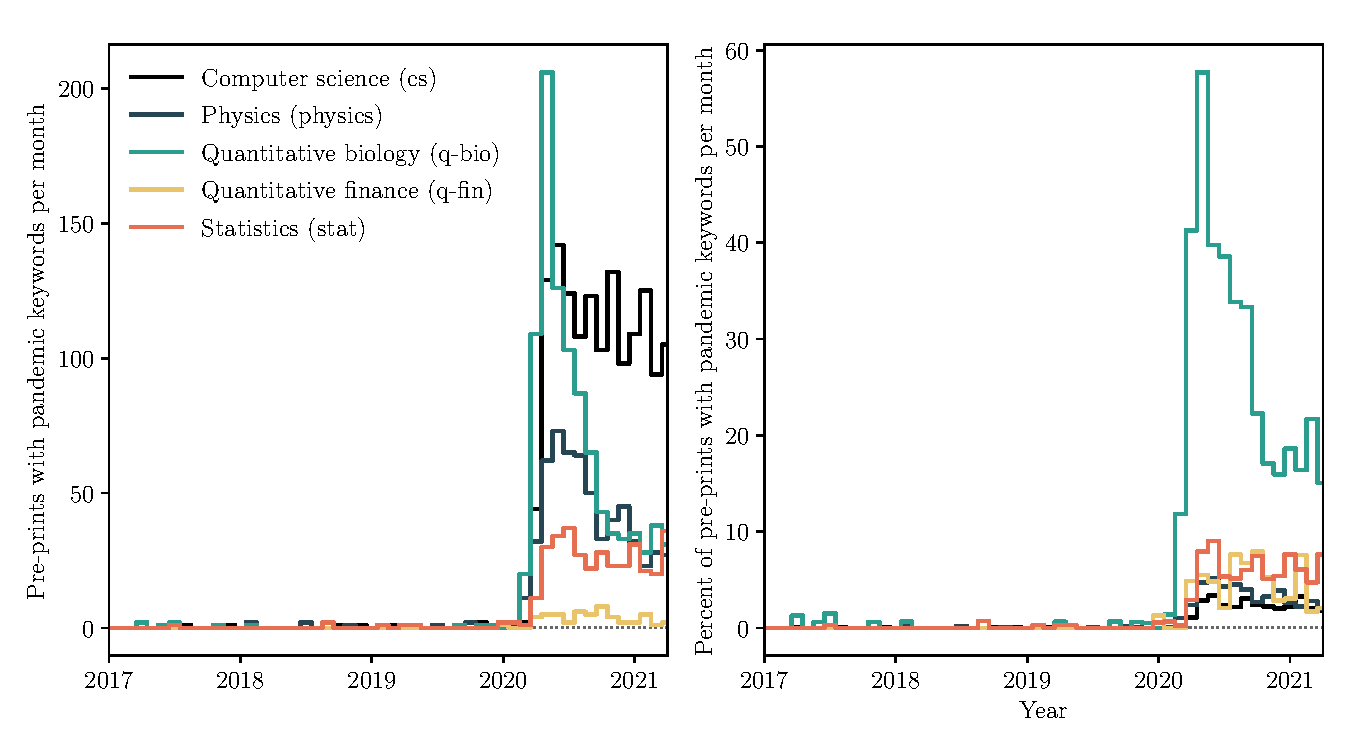
\includegraphics[width=\linewidth]{pandemic-related-preprints}
\caption{Pre-prints related to the COVID-19 pandemic peaked in April 2020, accounting for nearly 60\% the quantitative biology (\texttt{q-bio}) pre-prints in that month. Shown are five other research fields with the highest number of pandemic-related pre-prints in 2020. Monthly pre-prints are shown on the left, and the percent of pandemic-related pre-prints in that research field is shown on the right.}
\label{fig:2}
\end{figure}
 
\renewcommand{\thefootnote}{$\dagger$} 
 
An increase in quantitative biology\footnote{Quantitative biology is only a sub-field of biology, and most biology pre-prints are posted to bioRxiv ({https://biorxiv.org}).} research during a global pandemic is unsurprising. However, the question arises if this increase was driven by existing researchers in the field, or by authors from other fields entering quantitative biology due to the pandemic. In 2020 there was a peak in the number of new authors appearing for the first time in the quantitative biology literature (Figure~\ref{fig:3}) while the number of new authors in all other fields remained steady. The increase in pre-prints (and new authors) is driven by small (1-4) groups of authors, where many had never posted pre-prints to quantitative biology before.


\begin{figure}[!h]
\begin{center}
	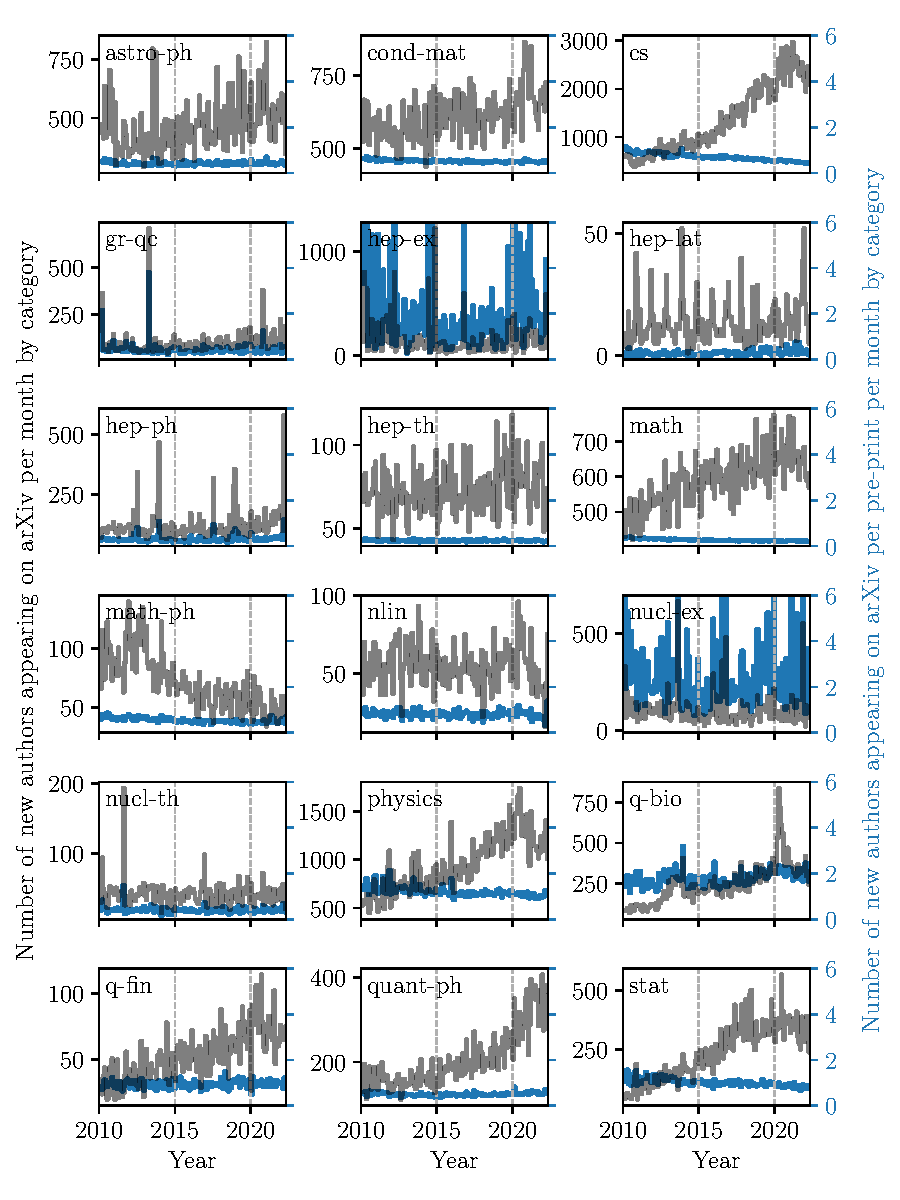
\includegraphics[width=0.95\linewidth]{new-authors-segmented-by-field-combined}
\end{center}
\caption{The number of new authors appearing in \arxiv\ pre-prints per month (grey) peaked in quantitative biology in 2020. Here we show new authors since 2010, but we used data since 2007 to determine if an author was new. The slow change in new authors  approximates the net number of new authors joining the field. The number of new authors appearing per number of pre-prints is shown in light blue, with identical limits on the right-hand y-axis. This highlights authorship differences between fields (e.g., \texttt{hep-ex} and \texttt{hep-lat}) for large experiments.}
\label{fig:3}
\end{figure}


One quarter of the excess pre-prints posted to quantitative biology during 2020 were both related to the pandemic and written by authors who had never appeared in the quantitative biology literature (234 of the 876 excess pre-prints in \texttt{q-bio}). A careful examination reveals that about half of these (45\%; 107/234) were written by mathematicians or physicists, with another 26\% (61/234) led by engineers, computer scientists, or economists. These pre-prints tend to focus on modelling the COVID-19 outbreak using public data sets, rather than quantitative biology research that requires more expert domain knowledge. About 3\% (8/234) were led by established biologists who have not used the \arxiv\ before and are now doing so presumably to help ensure that their COVID-19 research is more widely available. This fraction is likely higher among pre-prints where at least one author has appeared before in the quantitative biology literature. This represents a genuine increase in new researchers using the \arxiv, and a boost to making quantitative biology research more widely accessible. 

% What to say of the remaining 75%? 



%However, a careful examination of pandemic-related pre-prints in quantitative biology posted in 2020 shows that many were indeed written by researchers from other fields (primarily physicists and mathematicians), who had never posted about quantitative biology. 

%Some of these new authors in quantitative biology have never appeared in any other \arxiv\ fields before, either. A close examination of 234 pre-prints posted during 2020 to \texttt{q-bio.PE} where no authors had posted to \texttt{q-bio} before shows that 


%A close examination of these pre-prints reveals that many are  


% 234 papers in 2020 in q-bio.PE written about the pandemic where no author had ever appeared before in the q-bio literature.
% among these, 8 were led by authors who were domain experts in quantitative biology or a related field, and were 'new' to posting on arxiv
% among these 234, 107 (45%) were led by mathematicians or physicists, with another 61/234 (26%) led by engineers, computer scientists, or economists.

% [('mathematics', 58),
% ('physics', 41), + astrophysics, 8 ==> 49
% ('engineering', 26),
% ('computer science', 19),
% ('economics', 16),
% close examination of a random sample of 50 of these "new" authors and their academic affiliations found x to be established biologists who had not used the arXiv before while the rest were researchers from other fields (primarily physics and mathematics) who had not previously posted quantitative biology papers to the arXiv.

\newcommand{\totalcell}[1]{\cellcolor{gray!25}\textbf{#1}}

\begin{table}
       \caption{The number of \arxiv\ pre-prints per primary research field in 2020 and 2021, the percent change relative to 2019, predicted number of pre-prints using pre-pandemic data (see Methods), and the statistical significance between the predicted number and actual number of pre-prints.}
\begin{center}
\small
    \label{tab:table1}
    \begin{tabular}{|c|cccc|cccc|} 
    \hline
\arxiv\ & \multicolumn{4}{c|}{2020}  & \multicolumn{4}{c|}{2021} \\
primary & Actual & Change & Predicted & Sig. & Actual & Change & Predicted & Sig.  \\
category	& & (\%) &  &  $(\sigma)$ & & (\%) &  & $(\sigma)$ \\
%code &  &            & change (\%)&       & ($\sigma$)   &            & change (\%) &      & ($\sigma$) \\
\hline
astro-ph &  14,894 &  +3.4 &  14,990       & -0.1 &  14,388 &  -0.2 &  15,544        & -1.4 \\
%&         &       &  $\pm$   653 &      &         &       &   $\pm$   857 &      \\                
cond-mat &  16,187 &  +7.0 &  15,325       & +1.8 &  16,230 &  +7.3 &  15,561        & +1.0 \\
%&         &       &  $\pm$   492 &      &         &       &   $\pm$   644 &      \\                
cs &  54,802 & +24.3 &  51,669       & +0.8 &  61,396 & +39.3 &  59,433        & +0.3 \\
%&         &       &  $\pm$ 4,047 &      &         &       &   $\pm$ 5,698 &      \\                        
gr-qc &   3,404 & +12.3 &   3,166       & +1.5 &   3,521 & +16.2 &   3,316        & +1.0 \\
%&         &       &  $\pm$   154 &      &         &       &   $\pm$   201 &      \\                    
hep-ex &     615 & -19.8 &     818       & -2.2 &     828 &  +8.0 &     813        & +0.1 \\
%&         &       &  $\pm$    94 &      &         &       &   $\pm$   123 &      \\                    
hep-lat &     394 & -19.3 &     475       & -0.5 &     690 & +41.4 &     452        & +1.1 \\
%&         &       &  $\pm$   170 &      &         &       &   $\pm$   222 &      \\                
hep-ph &   4,585 &  +1.2 &   4,615       & -0.1 &   5,045 & +11.4 &   4,650        & +0.9 \\
%&         &       &  $\pm$   329 &      &         &       &   $\pm$   428 &      \\                    
hep-th &   3,870 &  +1.0 &   4,000       & -0.4 &   3,786 &  -1.2 &   4,163        & -1.0 \\
%&         &       &  $\pm$   291 &      &         &       &   $\pm$   379 &      \\                    
math &  35,367 &  +5.5 &  35,362       & +0.0 &  34,406 &  +2.6 &  37,091        & -1.6 \\
%&         &       &  $\pm$ 1,177 &      &         &       &   $\pm$ 1,640 &      \\                    
math-ph &   1,378 &  -6.3 &   1,460       & -0.9 &   1,117 & -24.0 &   1,468        & -2.8 \\
%&         &       &  $\pm$    95 &      &         &       &   $\pm$   124 &      \\                
nlin &     885 &  +6.1 &     822       & +1.0 &     787 &  -5.6 &     831        & -0.5 \\
%&         &       &  $\pm$    63 &      &         &       &   $\pm$    82 &      \\                    
nucl-ex &     499 &  +2.9 &     490       & +0.1 &     414 & -14.6 &     499        & -1.1 \\
%&         &       &  $\pm$    61 &      &         &       &   $\pm$    79 &      \\                
nucl-th &   1,212 &  -3.2 &   1,234       & -0.2 &   1,128 &  -9.9 &   1,223        & -0.7 \\
%&         &       &  $\pm$   111 &      &         &       &   $\pm$   144 &      \\                
physics &  15,242 & +14.3 &  14,746       & +1.0 &  13,917 &  +4.3 &  16,070        & -2.8 \\
%&         &       &  $\pm$   506 &      &         &       &   $\pm$   776 &      \\                
q-bio &   2,790 & +49.0 &   1,914       & +8.0 &   2,092 & +11.8 &   1,984        & +0.8 \\
%&         &       &  $\pm$   109 &      &         &       &   $\pm$   142 &      \\                    
q-fin &     979 & +23.1 &     805       & +3.2 &     850 &  +6.9 &     837        & +0.2 \\
%&         &       &  $\pm$    55 &      &         &       &   $\pm$    71 &      \\                    
quant-ph &   6,342 & +13.5 &   5,859       & +1.8 &   7,378 & +32.0 &   6,170        & +3.5 \\
%&         &       &  $\pm$   266 &      &         &       &   $\pm$   347 &      \\                
stat &   5,179 & +20.2 &   4,824       & +0.7 &   4,877 & +13.2 &   5,116        & -0.4 \\
%&         &       &  $\pm$   490 &      &         &       &   $\pm$   640 &      \\                    
\hline     
\totalcell{Total} & \totalcell{168,624} & \totalcell{+12.6} & \totalcell{162,574} & \totalcell{+1.4} & \totalcell{172,850} & \totalcell{+15.4} & \totalcell{175,221} & \totalcell{-0.4} \\
% \pm 4{,}393
% todo
\hline 
    \end{tabular}
  \end{center}
\end{table}


The pandemic has also created distinct challenges when interpreting trends in \arxiv\ data. For example, there was a large spike in papers submitted to the \texttt{stat} category in June 2020 which one might assume was driven by COVID-related work given what we have observed in \texttt{q-bio}. However, the number of COVID-related papers posted in this period is modest (Figure~\ref{fig:2}), and the key factor appears to be delayed paper submission deadlines for two large conferences (NeurIPS and the Joint Statistical Meetings). Both conferences have had submission deadlines in mid-May in recent years, but in 2020, their deadlines were moved to early June.


The COVID-19 pandemic appears to have had minimal impact on collective research productivity to date.
However, some significant changes were noted within specific areas of research. The largest persistent decline in pre-prints has occurred in {general physics (arXiv primary category \texttt{physics}), largely due to a decline in  pre-prints posted to computational and applied physics areas within the \texttt{physics} primary category. As of mid-2022, this steady decline continues.} Amongst individual fields the largest \emph{relative} decline in a single field is explainable by a high energy lattice physics conference that was cancelled in 2020. In this study we have only focussed on the quantity of publications as a measure for productivity, and not their quality. While citations are the most used measure of impact of academic publications, that metric becomes a more biased statistic when many related pre-prints are all being posted nearly at the same time\cite{Fassin:2021}. The relatively long timescales of academic research would suggest that the full impact on academic productivity due to the COVID-19 pandemic is yet to be seen. The methodology and results presented here provide a quantitative framework for future investigations of the longer term impacts of the pandemic.


\section*{Methods}

\subsection*{Grouping by research field}

Pre-prints posted to the \arxiv\ can be listed in a single field of research, or cross-listed in multiple fields. A field is annotated by \texttt{primary.SEC} where the primary field of research has the prefix, and the sub-field of research is represented by a short suffix. For example, one pre-print may have a primary field of research as stellar astrophysics (\texttt{astro-ph.SA}) and be cross-listed in machine learning (\texttt{stat.ML}). These field(s) of research are supplied by the corresponding author. It is a subjective decision whether to include more than one field of research, or what those fields of research would be. For this reason, throughout this work when we segment by research field we take the primary parent research field provided and ignore any cross-listed fields of research. When we segment pre-prints by sub-field, we similarly take the primary sub-field provided and ignore any cross-listings.

A pre-print's identifier is defined by the year and month that the pre-print was posted, and the number of pre-prints already posted in that month (across all fields). Pre-prints posted prior to April 2007 use a different identifier scheme, and a different research field definition. For these reasons, we have excluded pre-prints earlier than this date. 


\subsection*{Long-term modelling of monthly pre-print counts}

We use monthly pre-print counts per primary research field from January 2015 until December 2019 to make predictions for the number of pre-prints expected per month from January 2020 onwards. We use a straight line to model the mean pre-prints over time, and a Gaussian Process with a quasi-periodic kernel covariance function to capture seasonal periodicity\cite{Rasmussen:2006,Ambikasaran:2014}, and a white noise component. We fit the parameters of the mean model and the kernel hyper-parameters simultaneously, but kept the periodicity hyper-parameter fixed to one year. The predictions of the expectation and variance in the number of monthly pre-print counts are conditioned on the optimized hyper-parameters. We fit this model to monthly pre-print counts for every primary research field. These predictions are listed in Table~1. The expected total number of pre-prints, and the uncertainty in that number, are summed from the models used in individual research fields. 

Our conclusions are reasonably insensitive to the choice of model. As an alternative model we considered an autoregressive integrated moving average (ARIMA) model\cite{BoxJenkins:1970} with seasonal terms ($p=d=q=1$ for the non-seasonal component, and $P=D=Q=1$ with $m=12$ for the seasonal component). The predictions from the ARIMA model agree excellently with the mean predictions from the Gaussian Process model. The largest differences between these models is in \texttt{hep-lat}, where the ARIMA model predicts a higher peak number of pre-prints than the Gaussian Process model. This is not unexpected: the peak height of lattice physics pre-prints has been dropping for the last three years, and this gradual decline is better captured by the Gaussian Process model. If we adopted the ARIMA model then the drop in \texttt{hep-lat} pre-prints would become more significant. Throughout this work we adopt the predictions from the Gaussian Process model, unless otherwise specified.



\subsection*{Uniquely identifying authors}

The \arxiv\ team has parsed given and family names from author strings for all pre-prints. In general the author names have been appropriately parsed, even given a wide set of input formats. We made only one correction to these parsed names. When the author name was provided in the format of `Family-name First-given-name I.', without any commas, this was interpreted by the \arxiv\ parser such that the family name was `I.' and the given names were `Family-name First-given-name'. We identified situations like this by checking if the parsed family name was just an initial, and if two given names were parsed. In these situations, we correctly ordered the author name.

The \arxiv\ metadata available to us do not include institutional affiliations, or identifiers that would uniquely identify an author. 
There are two primary ways that name confusion could impact our inferences. In the first scenario, two people with the same name are amalgamated and treated as a single author that is on average twice as productive (or more, for very common names) as other authors. In the second scenario, an author will sometimes publish as `A.~B.~Smith', and other times publish as `A.~Smith'. A careful exploration of the data shows that this is a very frequent scenario, and if left uncorrected, would appear as many `unique' authors with half as many publications on average.

We have taken a simple approach to address name confusion. We first define a unique author by family name and the initial of the first given name (`Family-name, I.'), such that we intentionally group together authors that may share the same initial of their first given name. 
While our approach to name confusion is grossly simple, it is unlikely that these choices have any substantial impact on our inferences. In general, this errs on the side of name conflation and over-productivity, except for the relatively rare authors who change their last names over their career.
Any common name is likely to appear in the literature early in the data set and will not impact the conclusions we draw about how publishing changed from 2020 January onwards. Indeed, we re-produced the analysis and figures in this paper by taking all initials given and it made no change to our conclusions. This is due, in part, to most authors not providing middle initials.


\subsection*{Pre-prints related to the COVID-19 pandemic}

We identified a pre-print as being related to the COVID-19 pandemic if the title or abstract contained any of the following four (case-insensitive) terms: `pandemic', `COVID', `SARS-CoV-2', `lockdown', or `coronavirus'. Before 2020, these terms rarely appear in the title or abstract of any pre-print on \arxiv\ (Figure~\ref{fig:2}).




\vspace{\fill}


\ethics{No ethics approval was required for this work.}

\dataccess{All of the data and software used in this work are publicly available. The dataset used here is from \arxiv. The original dataset is curated by Cornell University and hosted by Kaggle (https://www.kaggle.com/Cornell-University/arxiv). The dataset is updated weekly. We accessed this dataset on 06 June 2022. We have stored a time-stamped version of this dataset, as well as the code used to process the data \cite{ZenodoRecord}.
A public GitHub repository (https://github.com/andycasey/arxiv) stores all software used to preprocess and analyse these data, including the scripts to produce the figures shown here, and to compile this manuscript. The repository includes a \texttt{README.md} file that describes the software environment used to perform the analysis, and steps on how to reproduce our work in full.}

\aucontribute{AC and IM conceived the idea to examine changes in academic productivity due to the pandemic. {PR} and IM helped guide the investigation and provided ideas on new avenues to explore and tests to perform. AC conducted the analysis. AC led the writing of the manuscript, with all authors contributing significantly. All authors read and iterated upon the text of the final manuscript.}

\competing{The authors declare no competing interests.}

\funding{A.~R.~C. is supported in part by the Australian Research Council through a Discovery Early Career Researcher Award (DE190100656). 
Parts of this research were supported by the Australian Research Council Centre of Excellence for All Sky Astrophysics in 3 Dimensions (ASTRO 3D), through project number CE170100013.
I.~M. is a recipient of the Australian Research Council Future Fellowship FT190100574.}

\ack{We thank Peter Skands (Monash University) 
	 and Ross Young (University of Adelaide) 
for comments on publication trends in high energy physics.
% Funding acknowledgements.
}

\disclaimer{The paper reflects the authors' views and may not reflect those of their employers, funding agencies, or affiliated institutions.}


\pagebreak

%%%%%%%%%% Insert bibliography here %%%%%%%%%%%%%%

\begin{thebibliography}{10}

\bibitem{Ginsparg:2011}
{Ginsparg}. P., {ArXiv at 20}, \emph{Nature}, \textbf{476}, 7359, doi:10.1038/476145a \newblock (2011).

\bibitem{Lariviere:2014}
{Larivi{\'e}re, V., et al.,} {arXiv E-prints and the journal of record: An analysis of roles and relationships}, \emph{Journal of the Association for Information Science and Technology}, \textbf{65}, 6, doi:10.1002/asi.23044 \newblock (2014).


\bibitem{Nicola:2020}
{Nicola, M., et al.,} {The socio-economic implications of the coronavirus pandemic ({COVID}-19): A review}, \emph{International Journal of Surgery}, \textbf{78}, 185--193, doi:10.1016/j.ijsu.2020.04.018 \newblock (2020).

\bibitem{Chu:2020}
{Yen-Hao Chu, I., Prima, A., Larson, H.~J., Leesa, L.}
{Social consequences of mass quarantine during epidemics: a systematic review with implications for the {COVID}-19 response}, \emph{Journal of Travel Medicine}, \textbf{27}, 7, doi:10.1093/jtm/taaa192 \newblock (2020).

\bibitem{IbnMohammed:2021}
{Ibn-Mohammed, T., et al.,} {A critical analysis of the impacts of {COVID}-19 on the global economy and ecosystems and opportunities for circular economy strategies}, \emph{Resources, Conservation and Recycling}, \textbf{164}, 105169, doi:1016/j.resconrec.2020.105169 \newblock (2021).


\bibitem{Viglione:2020}
{Viglione, G.}, {Are women publishing less during the pandemic? Here's what the data say}. \emph{Nature}, \textbf{581}, 356-366, doi:10.1038/d41586-020-01294-9 \newblock (2020).


\bibitem{Gewen:2020}
{Gewen, V.}, {The career cost of COVID-19 to female researchers, and how science should respond}. \emph{Nature}, \textbf{583}, 867--869, doi:10.1038/d41586-020-02183-x \newblock (2020).



\bibitem{King:2021}
{King, M.~M., Frederickson M.~E.}, {The Pandemic Penalty: The Gendered Effects of COVID-19 on Scientific Productivity}. \emph{Socius}. January 2021. doi:10.1177/23780231211006977 \newblock (2021).  


\bibitem{Clement:2019}
{Clement, C.~B., Bierbaum, M., O'Keeffe, K.~P., Alemi, A.~A.,}
{On the Use of ArXiv as a Dataset},
Preprint at https://arxiv.org/abs/1905.00075 \newblock (2019).

\bibitem{Rasmussen:2006}
{Rasmussen, C.~E., Williams, C.~K.~I.,}
{Gaussian Processes for Machine Learning}, \emph{MIT Press}, ISBN 026218253X \newblock (2016).

\bibitem{Ambikasaran:2014}
{Ambikasaran, S., Foreman-Mackey, D., Greengard, L., Hogg, D.~W., O'Neil, M.,}
{Fast Direct Methods for Gaussian Processes}, Preprint at http://arxiv.org/abs/1403.6015 \newblock (2014).

\bibitem{Guinnessy:2021}
Guinnessy, P. (Physics Today). 2021. \emph{Physicists gathered virtually for APS March Meeting}. [online] Available at {https://physicstoday.scitation.org/do/10.1063/PT.6.3.20210405a/full} [Accessed 17 June 2021].
 
\bibitem{LatticeConferenceWebsite}
Helmholtz-Institut f\"ur Strahlen- und Kernphysik Indico Service (Indico). 2021. \emph{The 38th International Symposium on Lattice Field Theory (Lattice 2020)}. [online] Available at: {https://indico.hiskp.uni-bonn.de/event/1/} [Accessed 3 June 2021].

\bibitem{LatticeConferenceWebsite2019}
Helmholtz-Institut f\"ur Strahlen- und Kernphysik Indico Service (Indico). 2021. \emph{The 38th International Symposium on Lattice Field Theory (Lattice 2020)}. [online] Available at: {https://indico.cern.ch/event/764552/} [Accessed 20 June 2022].

\bibitem{LatticeConferenceWebsite2021}
Helmholtz-Institut f\"ur Strahlen- und Kernphysik Indico Service (Indico). 2021. \emph{The 38th International Symposium on Lattice Field Theory (Lattice 2021)}. [online] Available at: {https://indico.cern.ch/event/1006302/} [Accessed 20 June 2022].

\bibitem{Wang:2017}
{Wang, W., Bai, X., Xia, F. et al.}, {From triadic closure to conference closure: the role of academic conferences in promoting scientific collaborations.}, \emph{Scientometrics}, \textbf{113}, 177–193  doi:10.1007/s11192-017-2468-x \newblock (2017).]

\bibitem{PhysicsWorld}
physicsworld (IOP Publishing). 2021. \emph{Critical research hit as COVID-19 forces physics labs to close}. [online] Available at {https://physicsworld.com/a/critical-research-hit-as-covid-19-forces-physics-labs-to-close/} [Accessed 4 June 2021].


\bibitem{ScienceMag}
Science Magazine (AAAS). 2021. \emph{Amid pandemic, Energy Department labs close to tens of thousands of users.} [online] Available at {https://www.sciencemag.org/news/2020/03/amid-pandemic-energy-department-labs-close-tens-thousands-users} [Accessed 4 June 2021].

\bibitem{Castelvecchi}
Castelvecchi, D. (Nature), {How the coronavirus pandemic is affecting the world's biggest physics experiments.} [online] Available at {https://www.nature.com/articles/d41586-020-00943-3} doi:10.1038/d41586-020-00943-3 [Accessed 6 June 2022].

\bibitem{Fassin:2021}
{Fassin, Y.} {Research on Covid-19: a disruptive phenomenon for bibliometrics}, \emph{Scientometrics}, \textbf{126}, 5305--5319, doi:10.1007/s11192-021-03989-w \newblock (2021).

\bibitem{BoxJenkins:1970}
{Box, G.~E.~P., Jenkins, G. M.} Time series analysis: Forecasting and control. San Francisco: Holden-Day. \newblock (1970).

\bibitem{ZenodoRecord} Casey, Andrew R. (2022). Impact of the COVID-19 pandemic on academic productivity [Data set]. Zenodo. https://doi.org/10.5281/zenodo.6615684

\end{thebibliography}

\end{document}
